\documentclass[11pt, oneside]{book}   	% use "amsart" instead of "article" for AMSLaTeX format
% !TEX encoding = UTF-8 Unicode
\usepackage[french,english]{babel}
\usepackage[T1]{fontenc}
\usepackage[utf8]{inputenc}


\usepackage[]{geometry} 

\usepackage{graphicx}
\setkeys{Gin}{width=\linewidth,totalheight=\textheight,keepaspectratio}
\graphicspath{{graphics/}}

	
\usepackage{amssymb}
\usepackage{tabularx}
\usepackage{mdwlist}
\usepackage{float}

\usepackage{hyperref}
\hypersetup{
	colorlinks = true,
	urlcolor = cyan
}

\usepackage{fancyvrb}
\fvset{fontsize=\normalsize}

\DefineVerbatimEnvironment{VerbatimText}{Verbatim}{frame=single,numbers=left,numbersep=2mm}
\DefineVerbatimEnvironment{VerbatimErl}{Verbatim}{frame=single,fontsize=\small}
\DefineVerbatimEnvironment{VerbatimEshell}{Verbatim}{frame=single,fontsize=\small}

\newcommand{\filename}[1]{\Verb`#1`}
\newcommand{\app}[1]{\Verb`#1`}
\newcommand{\otpapp}[1]{\Verb`#1`}
\newcommand{\module}[1]{\Verb`#1`}
\newcommand{\function}[1]{\Verb`#1`}
\newcommand{\expression}[1]{\Verb`#1`}
\newcommand{\command}[1]{\Verb`#1`}
\newcommand{\var}[1]{\Verb`#1`}

\def\includecode{\begingroup
\catcode`\_=12
\includecodeB}
\newcommand{\includecodeB}[2][erlang]{\VerbatimInput[frame=single,label=#1/#2,fontsize=\small]{#1/#2}\endgroup}



\title{Stuff Goes Bad:\protect\\ Erlang in Anger}
\author{
\includegraphics[width=150pt]{heroku-logo-light.pdf}\\
Fred Hébert}

\date{}							% Activate to display a given date or no date

\begin{document}
\maketitle

%%% Copyright page
\clearpage
\thispagestyle{empty}
\vspace*{\fill}



\begin{center}
\includegraphics[width=100pt]{by-nc-sa.eps}
\end{center}

\begin{center}
\emph{Erlang in Anger: Stuff Goes Bad} by Fred Hébert and Heroku is licensed under a \href{http://creativecommons.org/licenses/by-nc-sa/4.0/}{Creative Commons Attribution-NonCommercial-ShareAlike 4.0 International License}.
\end{center}

Thanks to additional work done by:

\emph{First Person's Name}, \emph{Second Person's Name}, ...

\vspace*{\fill}
\clearpage
%%%


\tableofcontents

\listoffigures

\chapter{Introduction}
\label{chap:introduction}

\section{On Running Software}
\label{sec:on-running-software}

There's something rather unique in Erlang in how it approaches failure compared to most other languages out there. In general, there's this kind of standard way of thinking where the language, programming environment, and methodology do everything possible to prevent errors. Something going wrong at run-time is something that needs to be prevented, and if it cannot be prevented, then it's out of scope for whatever solution people have been thinking about.

The program is written once, and after that, it's off to production, whatever may happen there.

Erlang, on the other hand, takes the approach that failures will happen no matter what, whether they're developer, operator, or hardware related. It is rarely practical or even possible to get rid of all errors in a program or a system.\footnote{life-critical systems are usually excluded from this category, but some cases still happen.} The idea quickly becomes that if you can deal with some errors rather than preventing them at all cost, then most undefined behaviours of a program can go in that "deal with it" approach.

This is where the "Let it Crash"\footnote{Erlang people now seem to favour "let it fail", given it makes people far less nervous.} idea comes from: Because you can now deal with failure, and because the cost of weeding out all of the complex bugs from a system before it hits production is often prohibitive, the programmer should only deal with the errors he or she knows how to handle, and leave the rest for another process (a supervisor) or the virtual machine to deal with.

Given most bugs are transient\footnote{131 out 132 bugs are transient bugs (they're caused by circumstances, and restarting them may solve the problem entirely), according to Jim Gray in \href{http://www.hpl.hp.com/techreports/tandem/TR-85.7.html}{Why Do Computers Stop and What Can Be Done About It?}}, just restarting faulty processes from a state known to be stable will be surprisingly good at dealing with errors.

If I'm allowed an analogy, Erlang is a programming environment where what you have is equivalent to the human body's immune system, whereas most other languages only care about hygiene to make sure no germ enters the body. Both forms appear extremely important to me. Pretty much every environment offers the hygiene, to varying degrees. Nearly no other environment offers the immune system.

Because the system doesn't collapse the first time something bad touches it, Erlang/OTP also allows you to be a doctor. You can go in the system, pry it open, carefully observe everything inside as it runs, and even try to fix it interactively. To continue with the analogy, Erlang allows you to perform extensive tests to diagnose the problem and various degrees of surgery (even very invasive surgery), without the patient needing to sit down or interrupt his daily activities.

This book intends to be a little guide about how to be the Erlang medic in a time of war. It is first and foremost a collection of tips and tricks to help understand where failures come from, and a dictionary of different code snippets and practices that helped developers debug production systems that were built in Erlang.

\section{Who is this for?}
\label{sec:who-is-this-for}

This book is not a book for absolute beginners. There is usually a gap left between most tutorials, books, training sessions, and actually being able to deliver a product that works. There's a fumbling phase implicit to a programmer's learning of a new language an environment, where you just have to figure how to get out of the guidelines and step into the real world, with the community that goes with it.

This book thus assumes that the reader is somewhat proficient in basic Erlang and the OTP framework, but doesn't make an assumption to what extent. Erlang/OTP features are explained as I see fit -- usually when I consider them tricky -- and it is expected that a reader who feels confused by usual Erlang/OTP material will have an idea of where to look for explanations if necessary\footnote{I do recommend visiting \href{http://learnyousomeerlang.com}{Learn You Some Erlang} or the regular \href{http://www.erlang.org/erldoc}{Erlang Documentation} if a free resource is required}.

What is not assumed is that the reader necessarily knows how to debug Erlang software, dive in an existing code base, diagnose issues, or has an idea of some of the best practices about deploying Erlang in a production environment\footnote{Running Erlang in a screen or tmux session is \emph{not} a deployment strategy.}.

\section{How To Read This Book}
\label{sec:how-to-read-this-book}

I HAVE NO IDEA YET

%%%
%%%
%%%

\part{Writing Applications}
\label{part:writing-applications}

\chapter{How to Dive in a Code Base}
\label{chap:how-to-dive-in-a-code-base}

"Read the source" is one of the most annoying thing to be told, but dealing with Erlang programmers, you'll have to do it plenty of times. Either the documentation for a library will be incomplete, outdated, or just not there. In other cases, Erlang programmers are a bit similar to Lispers in that they will tend to write libraries that will solve their problems, and not really test or try them in other circumstances, leaving it for you to extend or fix issues that arise in new contexts.

It's thus pretty much guaranteed you'll have to go dive in some code base you know nothing about, either because you inherited it at work, or because you need to fix it or understand it to be able to move forward with your own system. This is in fact true of most languages whenever the project you work on is not one you architected yourself.

There are three main types of Erlang code bases you'll encounter in the wild: raw Erlang code bases, OTP applications, and OTP releases. In this chapter, we'll look at each of these and try to provide helpful tips on navigating them.

\section{Raw Erlang}
\label{sec:dive-raw-erlang}

If you encounter a raw Erlang code base, you're pretty much on your own. These rarely follow any specific standard, and you have to dive in the old way to figure out whatever happens in there.

This means hoping for a \filename{README.md} file or something similar that can point to an entry point in the application, and going from there, or hoping for some contact information that can be used to ask questions to the author(s) of the library.

Fortunately, you should rarely encounter raw Erlang in the wild, and you will know early on they are often beginner projects, or awesome projects that were once built by Erlang beginners and now would need a serious rewrite. In general, the advent of tools such as \app{rebar}\footnote{a build tool briefly introduced in Chapter \ref{chap:building-open-source-erlang-software}} made it so most people use OTP Applications, even where not appropriate.

\section{OTP Applications}
\label{sec:dive-otp-applications}

Figuring out OTP applications is usually rather simple. They usually all share a directory structure that looks like:

\begin{VerbatimText}
doc/
ebin/
src/
test/
LICENSE.txt
README.md
rebar.config
\end{VerbatimText}

There might be slight differences, but the general structure will be the same.

Each OTP application should contain an \emph{app file}, either \filename{ebin/<AppName>.app} or more often, \filename{src/<AppName>.app.src}\footnote{a build system generates the final file that goes in \filename{ebin}. Note that in these cases, many  \filename{src/<AppName>.app.src} files do not specify modules and let the build system take care about it.}. There are two main varieties of app files:

\includecode[erlang]{useragent.app.src}

And:

\includecode[erlang]{dispcount.app}

This first case is called a \emph{library application}, while the latter case is a regular \emph{application}.

\subsection{Library Applications}
\label{subsec:dive-library-applications}

Library applications will usually tend to have a bunch of modules named \module{appname\_something}, and one module named \module{app\_name}. This will usually be the interface module that's central to the library and contains a quick way into most of the functionality to be provided.

By looking at the source of the module, you can figure out how it works with little effort: If there's any given behaviour in there (\module{gen\_server}, \module{gen\_fsm}, etc.), you're most likely expected to start a process under one of your own supervisors and call it that way. If there isn't, then you probably have a functional library on your hands.

\subsection{Regular Applications}
\label{subsec:dive-regular-applications}

For a regular OTP application, there are two potential files that act as the entry point:

\begin{enumerate*}
	\item \module{appname}
	\item \module{appname\_app}
\end{enumerate*}

The first file should be similar in use to what we had in a library application (an entry point), while the second one will implement the \module{application} behaviour, and will represent the top of the application's process hierarchy. In some cases the first file will play both roles at once.

If you plan on using the application, look inside \module{appname} for details and information. If you need to maintain and/or fix the application, go for \module{appname\_app} instead.

The application will necessarily start a top-level supervisor and return its \expression{pid}. This top-level supervisor will then contain the specifications to all the children it will start on its own\footnote{In some cases, the supervisor specifies no child: they will either be started dynamically by some function of the API or in a start phase of the application, or the supervisor is only there to allow OTP environment variables (in the \expression{env} tuple of the app file) to be loaded.}.

The higher a process resides in the tree, the more likely it is to be vital to the survival of the application. You can also estimate how important a process is by the order it is started (all children are started in order, depth-first). If a process is started later in the supervision tree, it probably depends on ones that were started earlier.

Moreover, worker processes that depend on each other within the same application (say, a process that buffers socket communications and relays them to a finite-state machine in charge of understanding the protocol) are likely to be regrouped under the same supervisor and to fail together when something goes wrong. This is a deliberate choice, as it is usually simpler to start from a blank slate with both processes rather trying to figure out how to recuperate when one or the other loses or corrupts its state.

The supervisor restart strategy will usually determine how these go together:

\begin{itemize*}
	\item \expression{one\_for\_one} and \expression{simple\_one\_for\_one} are used for processes that are not depending on each other directly, although their failures will collectively counted towards total application shutdown\footnote{Some developers will use \expression{one\_for\_one} supervisors when \expression{rest\_for\_one} is more appropriate. They will require the order to boot correctly, but forget about said order when restarting or if a predecessor dies.}.
	\item \expression{rest\_for\_one} will be used to represent processes that depend on each other in a linear manner.
	\item \expression{one\_for\_all} is used for processes that entirely depend on each other.
\end{itemize*}

Because of this, it is easiest to navigate OTP applications in a top-down manner by exploring supervision subtrees. 

For each worker process supervised, the behaviour it implements will give a good clue about its purpose:

\begin{itemize*}
	\item a \module{gen\_server} holds resources and tends to follow client/server patterns (or more generally, request/response patterns)
	\item a \module{gen\_fsm} will deal with a sequence of events or inputs and react depending on them, as a Finite State Machine. It will often be used to implement protocols.
	\item a \module{gen\_event} will act as an event hub for callbacks, or as a way to deal with notifications of some sort.
\end{itemize*}

All of these modules will contain the same kind of structure: exported functions that represent the user-facing interface, exported functions for the callback module, and private functions.

Based on their supervision relationship and the typical role of each behaviour, looking at the interface to be used by other module and the behaviour implemented should reveal a lot of information about the program you're diving in.

\subsection{Dependencies}
\label{subsec:dive-dependencies}

All applications have dependencies (at the very least on the \module{kernel} and \module{stdlib} applications), and these dependencies will have their own dependencies. OTP applications usually share no state between them, so it's possible to know what bits of code depend on what other bits of code by looking at the app file only, assuming the developer wrote them in a mostly correct manner. Figure~\ref{fig:app-deps} shows a diagram that can be generated from looking at app files to help understand the structure of OTP applications.


\begin{figure}
  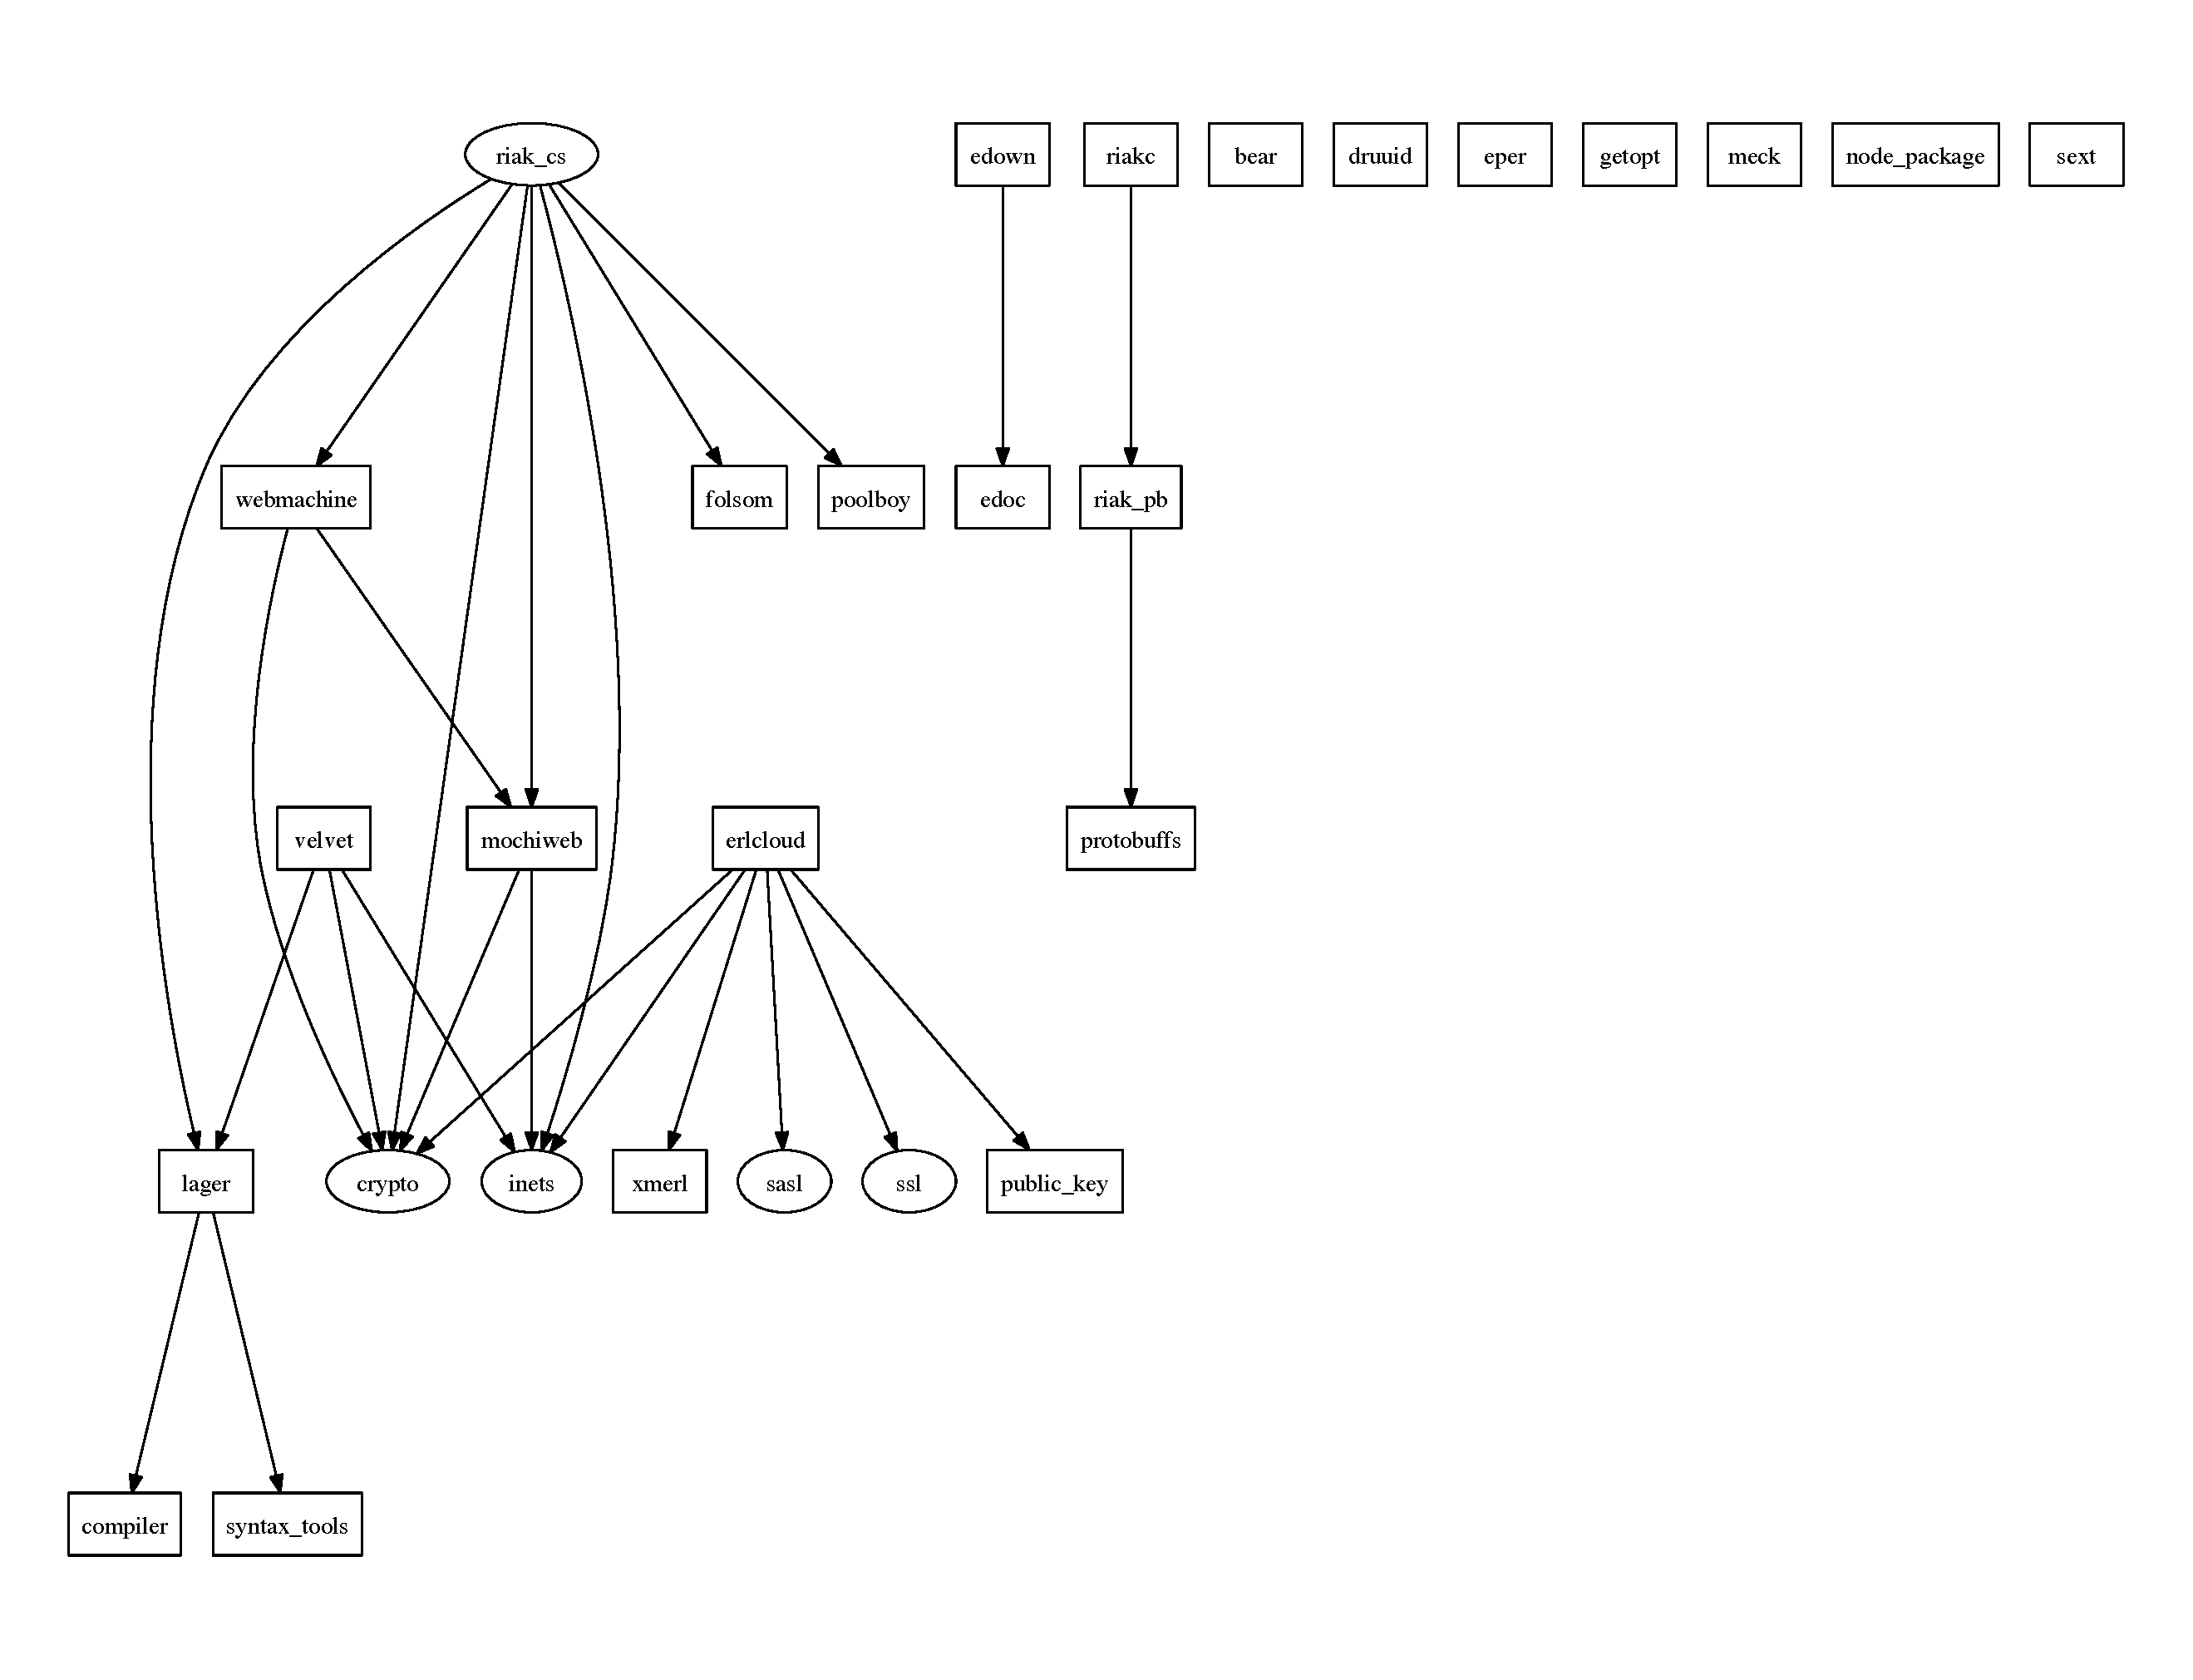
\includegraphics{app-deps-riak-cs.pdf}%
  \caption{Dependency graph of riak\_cs, Basho's open source cloud library.
  The graph has been generated with app\_deps, shown in \ref{chap:app-deps}}%
  \label{fig:app-deps}%
\end{figure}

Using such a hierarchy and looking at each application's short description might be helpful to draw a rough, general map of where everything is located. Similar hierarchies can be found using the \module{observer}\footnote{\href{http://www.erlang.org/doc/apps/observer/observer\_ug.html}{http://www.erlang.org/doc/apps/observer/observer\_ug.html}} application, but for individual supervision trees. Put together, you may get an easy way to find out what does what in the code base.

\section{OTP Releases}
\label{sec:dive-otp-releases}

OTP releases are not a lot harder to understand than most OTP Applications in the wild. A release is a set of OTP applications packaged in a production-ready manner so it boots and shuts down without needing to manually call \function{application:start/2} for any app. Of course there's a bit more to release than that, but generally, the same discovery process used for individual OTP Applications will be applicable here.

You'll usually have a file similar to the configuration files used by \module{systools} or \module{reltool}, which will state all applications part of the release and a few\footnote{a lot} options regarding their packaging. To understand them, I recommend \href{http://learnyousomeerlang.com/release-is-the-word}{reading existing documentation on them}. If you're lucky, the project may be using \app{relx}\footnote{\href{https://github.com/erlware/relx/wiki}{https://github.com/erlware/relx/wiki}}, an easier tool that recently appeared.

%%%
%%%
%%%

\chapter{Building Open Source Erlang Software}
\label{chap:building-open-source-erlang-software}

Most Erlang books tend to explain how to build Erlang and OTP applications, but few of them go very much in depth about how to integrate with the Erlang community doing Open Source work. Some of them avoid the topic on purpose. This chapter dedicates itself to doing a quick tour of the state of affair in Erlang.

OTP Applications are the vast majority of the open source code people will encounter. In fact, many people who would need to build an OTP release would do so as one umbrella OTP Application. 

If what you're writing is a stand-alone piece of code that could be used by someone building a product, it's likely an OTP Application. If what you're building is a product that stands on its own and should be deployed by users as-is (or with a little configuration), what you should be building is an OTP release\footnote{The details of how to build and OTP Application or release is left up to the Erlang introduction book you have at hand}.

The main build tools supported are \app{rebar} and \app{erlang.mk}. The former is a portable Erlang script that will be used to wrap around a lot of standard functionality and add its own, while the latter is a very fancy makefile that does a bit less, but tends to be faster when it comes to compiling. In this chapter, I'll mostly focus on using \app{rebar}\footnote{\href{https://github.com/rebar/rebar}{https://github.com/rebar/rebar}} to build things, given it's the ad-hoc standard, is well-established, and \app{erlang.mk} applications tend to also be supported by \app{rebar} as dependencies.

\section{Project Structure}
\label{sec:project-structure}

The structure of OTP applications and of OTP releases are different. An OTP application can be expected to have one top-level supervisor (if any) and possibly a bunch of dependencies that sit below it. An OTP release will usually be composed of multiple OTP applications, which may or may not depend on each other. This will lead to two major ways to lay out applications.

\subsection{OTP Applications}
\label{subsec:building-otp-applications}

For OTP applications, the proper structure is pretty much the same as what was explained in \ref{sec:dive-otp-applications}:

\begin{VerbatimText}
doc/
deps/
ebin/
src/
test/
LICENSE.txt
README.md
rebar.config
\end{VerbatimText}

What's new in this one is the \filename{deps/} directory, which is fairly useful to have, but that will be generated automatically by \app{rebar}\footnote{A lot of people package \app{rebar} directly in their application. This was initially done to help people who never used rebar before use libraries and projects in a boostrapped manner. Feel free to install rebar globally and your system and use that, if you want to.} if necessary. That's because there is no canonical package management in Erlang. People instead use whatever \app{rebar} decided, which was that you fetch dependencies locally. This is fine and removes a truckload of conflicts, but means that each project you have may have its own set of dependencies.

This is decided in \app{rebar} by adding a few config lines to \filename{rebar.config}:

\begin{VerbatimText}
{deps,
 [{application_name, "1.0.*",
   {git, "git://github.com/user/myapp.git", {branch,"master"}}},
  {application_name, "2.0.1",
   {git, "git://github.com/user/hisapp.git", {tag,"2.0.1"}}},
  {application_name, "", 
   {git, "https://bitbucket.org/user/herapp.git",  "7cd0aef4cd65"}},
  {application_name, "my regex",
   {hg, "https://bitbucket.org/user/theirapp.hg" {branch, "stable"}}}]}.
\end{VerbatimText}

Applications are fetched directly from a \app{git} (or \app{hg}, or \app{svn}) source, recursively. They can then be compiled, and specific compile options can be added with the \expression{\{erl\_opts, List\}.} option in the config file\footnote{More details by calling \command{rebar help compile}}. 

Within these directories, you can do your regular development of an OTP Application. To compile them, calling \command{rebar get-deps compile} will go download all dependencies, and then build them and your app at once.

When making your application public to the world, distribute it \emph{without} the dependencies. It's quite possible other developers' own applications have dependencies on the same applications yours do, and it's no use shipping them all multiple times. The build system in place (in this case, \app{rebar}) should be able to figure out duplicated entries and fetch everything necessary only once.

%% erlang.mk downloads relx for releases, and runs it iff there's a relx file there

\subsection{OTP Releases}
\label{subsec:building-otp-releases}

For releases, the structure should be a bit different\footnote{I say \emph{should} because many Erlang developers put their final system under a single top-level application (in \filename{src}) and a bunch of follower ones as dependencies (in \filename{deps}), which is less than ideal for distribution purposes. People who do that tend to build from source on the production servers and run custom commands to boot their applications.}. Because releases are collections of applications, their structure should reflect that.

Instead of having a top-level app, most applications should be equal. Then, a useful distinction to have is to have a directory for the applications' source code currently being contained within the existing repository (say, internal business code), and another one for dependencies (which are managed independently).

\begin{VerbatimText}
apps/
doc/
deps/
LICENSE.txt
README.md
rebar.config
\end{VerbatimText}

This structure will allow to then generate releases. Tools such as Systool and Reltool have been covered before\footnote{\href{http://learnyousomeerlang.com/release-is-the-word}{http://learnyousomeerlang.com/release-is-the-word}}, and can allow the user plenty of power. An easier tool that recently appeared is \app{relx}\footnote{\href{https://github.com/erlware/relx/wiki}{https://github.com/erlware/relx/wiki}}.

A configuration file for the directory structure above would look like:

\begin{VerbatimText}
{paths, ["apps", "deps"]}.
{include_erts, false}. % will use currently installed Erlang
{default_release, demo, "1.0.0"}.

{release, {demo, "1.0.0"},
    [members,
     feedstore,
     ...
     eper,
     recon]}.
\end{VerbatimText}

Calling \command{./relx} (if the executable is in the current directory) will build a release, to be found in a \filename{\_rel/} directory. If you really like using \app{rebar}, you can make the release-building part of the compilation by using a rebar hook in \filename{rebar.config}:

\begin{VerbatimText}
{post_hooks,[{compile, "./relx"}]}.
\end{VerbatimText}

And every time \command{rebar compile} will be called, the release will be generated.

\section{Supervisors and start\_link Semantics}
\label{sec:supervisors-and-start-link-semantics}

In complex production systems, most faults and errors are going to be transient, and retrying an operation will be a good way to do things — Jim Gray's paper\footnote{\href{http://mononcqc.tumblr.com/post/35165909365/why-do-computers-stop}{http://mononcqc.tumblr.com/post/35165909365/why-do-computers-stop}} quotes Mean Times Between Failures of systems handling transient bugs being better by a factor of 4. Still, supervisors aren't just about restarting.

One very important part of Erlang supervisors and their supervision trees is that their start phase is synchronous. Each OTP Process started has a period during which it can do its own thing, preventing the entire boot sequence of its siblings and cousins to come. If the process dies there, it's retried again, and again, until it works, or fails too often.

That's where people make a very common mistake. There isn't a backoff or cooldown period before a supervisor restarts a crashed child. When people write a network-based application and try to set up a connection in this initialization phase, and that the remote service is down, the application fails to boot after too many fruitless restarts. Then the system may shut down.

Many Erlang developers end up arguing in favor of a supervisor that has a cooldown period. I strongly oppose the sentiment for one simple reason: it's all about the guarantees.

\subsection{It's About the Guarantees}
\label{subsec:start-link-guarantees}

Restarting a process is about bringing it back to a stable, known state. From there, things can be retried. When the initialization isn't stable, supervision is worth very little. An initialized process should be stable no matter what happens. That way, when its siblings and cousins get started later on, they can be booted fully knowing that the rest of the system that came up before them is healthy.

If you don't provide that stable state, or if you were to start the entire system asynchronously, you get very little benefit from this structure that a \expression{try ... catch} in a loop wouldn't provide.

Supervised processes \emph{provide guarantees} in their initialization phase, \emph{not a best effort}. This means that when you're writing a client for a database or service, you shouldn't need a connection to be established as part of the initialization phase unless you're ready to say it will always be available no matter what happens.

You could force a connection during initialization if you know the database is on the same host and should be booted before your Erlang system, for example. Then a restart should work. In case of something incomprehensible and unexpected that breaks these guarantees, the node will end up crashing, which is desirable: a pre-condition to starting your system hasn't been met. It's a system-wide assertion that failed.

If, on the other hand, your database is on a remote host, you should expect the connection to fail. In this case, the only guarantee you can make in the client process is that your client will be able to handle requests, but not that it will communicate to the database. It could return \expression{\{error, not\_connected\}} on all calls during a net split, for example.

The reconnection to the database can then be done using whatever cooldown or backoff strategy you believe is optimal, without impacting the stability of the system. It can be attempted in the initialization phase as an optimization, but the process should be able to reconnect later on if anything ever disconnects.

If you expect failure to happen on an external service, do not make its presence a guarantee of your system. We're dealing with the real world here, and failure of external dependencies is always an option. To put it another way, we're going to lean on liveness (something good should eventually happen) as a guarantee, and reduce the safety (something bad will never happen) that we promise when it comes to the availability of services in a distributed system.

\subsection{Side Effects}
\label{subsec:start-link-side-effects}

Of course, the libraries and processes that call such a client will then error out if they didn't expect to work without a database. That's an entirely different issue in a different problem space, but not one that is always impossible to work around. For example, let's pretend the client is to a statistics service for Ops people — then the code that calls that client could very well ignore the errors without adverse effects to the system as a whole. 

The difference in both initialization and supervision approaches is that the client's callers make the decision about how much failure they can tolerate, not the client itself. That's a very important distinction when it comes to designing fault-tolerant systems. Yes, supervisors are about restarts, but they should be about restarts to a stable known state.

\subsection{Example: Initializing without guaranteeing connections}
\label{subsec:start-link-initializing-without-guaranteeing-connections}

So instead of doing:

\begin{VerbatimText}
init(Args) ->
    Opts = parse_args(Args),
    {ok, Port} = connect(Opts),
    {ok, #state{sock=Port, opts=Opts}}.

[...]

handle_info(reconnect, S = #state{sock=undefined, opts=Opts}) ->
    case connect(Opts) of
        {ok, New} -> {noreply, S#state{sock=New}};
         _ -> self() ! reconnect, {noreply, S}
    end;
\end{VerbatimText}

Which would guarantee a given connection as part of the process' state (even though it may be ready to handle a failure of said connection). The function could be rewritten as:

\begin{VerbatimText}
init(Args) ->
    Opts = parse_args(Args),
    %% you could try connecting here anyway, for a best
    %% effort thing, but be ready to not have a connection.
    self() ! reconnect,
    {ok, #state{sock=undefined, opts=Opts}}.

[...]

handle_info(reconnect, S = #state{sock=undefined, opts=Opts}) ->
    case connect(Opts) of
        {ok, New} -> {noreply, S#state{sock=New}};
        _ -> self() ! reconnect, {noreply, S}
    end;
\end{VerbatimText}

And allow initializations with fewer guarantees: they went from \emph{the connection is available} to \emph{the connection manager is available}.

\subsection{In a nutshell}
\label{subsec:start-link-in-a-nutshell}

Production systems I end up working with often end up being a mix of both approaches.

Things like configuration files, accessibility to the file system (say for logging purposes), local resources that can be depended on (opening UDP ports for logs), restoring a stable state from disk or network, and so on, are things I'll readily put into requirements of a supervisor and may decide to synchronously load no matter how long it takes (some applications may just end up having over 10 minutes boot times in rare cases, but that's okay because we're possibly syncing gigabytes that we \emph{need} to work with as a base state if we don't want to serve incorrect information.)

On the other hand, code that depends on non-local databases and external services will have the partial startup with quick tree booting because if the failure is expected to happen often during regular operations,
then there's no difference between now and later. You have to handle it the same, and for these parts of the system, far less strict guarantees are often the solution.

\subsection{Application Strategies}
\label{subsec:start-link-application-strategies}

No matter what, a sequence of failures is not a death sentence for the node. Once a system has been divided in various OTP applications, it becomes possible choose which application is vital or not to the node. Each OTP application can be started in 3 ways: temporary, transient, permanent, either by doing it manually in \expression{application:start(Name, Type)}, or in the config for releases in systools or reltool:

\begin{itemize*}
	\item permanent: if the app terminates, the entire system is taken down, excluding manual termination of the app with \function{application:stop/1}.
	\item transient: if the app terminates for reason 'normal', that's ok. Any other reason for termination shuts down the entire system.
	\item temporary: the application is allowed to stop for any reason. It will be reported, but nothing bad will happen.
\end{itemize*}

Nothing in there says "OTP shuts down the node all the time" nearly as much as the configuration given to it.


%%%
%%%
%%%

\chapter{Planning for Overload}

By far the most common cause of failure I've encountered in real-world scenarios were about the node going out of memory, and usually having this related to message queues going out of bounds.\footnote{Figuring out that a message queue is the problem is explained in INSERT REFERENCE HERE} There are plenty of ways to deal with this, but knowing which one to use will require a decent understanding of the system you're working on.

To oversimplify things, most of the projects I end up working on can be visualized as a very large toilet. User and data input are how much crap go in the toilet. The Erlang system itself is the pipe, and wherever the output goes is the sewer system.

When an Erlang node dies because of a queue going out, figuring out who to blame is crucial. Did someone put too much crap in the toilet? Are the sewer systems backing up? Did you just design too small a pipe?

Determining what queue blew up is not necessarily hard. This is information that can be found in a crash dump. Finding out why it blew up is trickier. Based on the role of the process or run-time inspection, it's possible to figure out whether causes include fast flooding, blocked processes that won't process messages fast enough, and so on.

The most difficult part is to decide how to fix it. When the toilet gets clogged up by too much waste, we will usually start by trying to make the pipe (our program) larger. Then the crap gets pushed further down the system, until the sewers can't take it anymore. At that point, we may try to add toilets or various locations to help with global input of crap.

Then there's a point where things can't be improved anymore at the toilet's level. There are too many logs\footnote{tee hee} sent around, there's a bottleneck on databases that \emph{need} the consistency, or there's simply not enough knowledge or manpower in your organization to improve things there.

We need to be more clever, and so things are moved back up a level. We try to massage the information going in the system to make it either lighter (whether it is through compression, better algorithms and data representation, caching, and so on). Even then, there are times where overload will be too much, and we have to make the hard decisions between restricting the input to the system, discarding it, or accepting that the system will reduce its quality of service up to the point it will crash.

In this section, we will explore common causes of queues blowing up and overload in Erlang systems, with possible solutions.

\section{error\_logger Explodes}

Ironically, the process in charge of error logging is one of the most fragile ones. In a default Erlang install, the \module{error\_logger}\footnote{defined at \href{http://www.erlang.org/doc/man/error\_logger.html}{http://www.erlang.org/doc/man/error\_logger.html}} process will take its sweet time to log things to disk or over the network, and will do so much more slowly than errors can be generated.

This is especially true of user-generated log messages (not for errors), and for crashes in large processes. For the former, this is because \module{error\_logger} doesn't really expect arbitrary levels of messages coming in continually. It's for exceptional cases only and didn't expect lots of traffic. For the later, it's because the entire state of processes (including their mailboxes) get copied over to be logged. It only takes a few of them to have memory bubbling up a lot, and if it's not enough to cause the node to go Out Of Memory (OOM), it may slow the logger enough that additional messages will.

The best solution for this at the time of writing is to use \href{https://github.com/basho/lager}{\module{lager}} as a substitute logging library.

While Lager will not solve all your problems, it will truncate voluminous log messages, optionally drop off OTP-generate error messages when they go over a certain threshold, and will automatically switch between asynchronous and synchronous modes for user-submitted messages in order to self-regulate.

It won't be able to deal with very specific cases, where user-submitted messages are in high volume and all coming from one-off processes. This is, however, a much rarer occurrence than everything else, and one where the programmer tends to have more control.


\section{Locks and Blocking Operations}

Locking and blocking operations will often be problematic when they're taking unexpectedly long to execute in a process that's constantly being piled on by tasks.

One of the most common example I've seen is a process blocking while accepting a connection or waiting for messages with TCP sockets. During blocking operations of this kind, messages are free to pile up in the message queue.

One particular bad example I've seen was in a pool manager for HTTP connections that I had written in a fork of the \href{https://github.com/ferd/lhttpc}{\module{lhttpc}} library. It worked fine in most test cases we had, and we even had a connection timeout set to 10 milliseconds to be sure it never took too long\footnote{10 milliseconds is very short, but was fine for collocated servers used for real-time bidding.}. It had a few weeks of perfect uptime when it suddenly got to be very bad and killed a node or degraded performance in unacceptable ways.

The reason behind this degradation was that when the remote server would go down, all of a sudden, all connecting operations would take at least 10 milliseconds, the time before which the connection attempt is given up on. With around 9,000 messages per second to the central process, each usually taking under 5 milliseconds, the impact became similar to roughly 18,000 messages a second and things got out of hand.

The solution we came up with was to leave the task of connecting to the caller process, and enforce the limits as if the manager had done it on its own. All of a sudden, the blocking operations were distributed to all users of the library, and even less work was required to be done by the manager, now free to accept more requests.

The general lesson to remember from such cases is that when there is \emph{any} point of your program that ends up being a central hub, receiving messages, any lengthy task should be moved out of there if possible. Tutorials tend to tell new Erlang programmers to use processes only for truly concurrent tasks and to not put them everywhere just for the sake of it. Handling predictable overload\footnote{Something you know for a fact gets overloaded in production} situations by adding more processes -- which either handle the blocking operations or instead act as a buffer while the "main" process blocks -- is often a good idea.

There will be an increased complexity in managing more processes for activities that aren't technically concurrent, so make sure you really need them before programming defensively.

Another option is to transform the blocking task into an asynchronous one. If the type of work allows it, start the long-running job and keep a token that identifies it uniquely, along with the original requester you're doing work for. When the resource is available, have it send a message back to the server with the aforementioned token. The server will eventually get the message, match the token to the requester, and answer back, without being blocked by other requests in the mean time.\footnote{The \otpapp{redo} application is an example of a library doing this, in its \href{https://github.com/JacobVorreuter/redo/blob/master/src/redo\_block.erl}{redo\_block} module. The [under-documented] module turns a pipelined connection into a blocking one, but does so while maintaining pipeline aspects to the caller -- this allows the caller to know that only one call failed when a timeout occurs, not all of the in-transit ones, without having the server stop accepting requests.}.

This option tends to be more obscure than using many processes and can quickly devolve into callback hell, but may use fewer resources.

\section{Unexpected Messages}

Messages you didn't know about tend to be rather rare when using OTP applications. Because OTP behaviours pretty much expect you to handle anything with some clause for \function{handle\_info/2}, unexpected messages will not accumulate much.

However, all kinds of OTP-compliant systems end up having processes that may not implement a behaviour, or goes in a non-behaviour stretch where it overtakes message handling. If you're lucky enough, monitoring tools\footnote{REF HERE} will show a constant memory increase, and inspecting for large queue sizes\footnote{REF HERE} will let you find which process is at fault. You can then fix the problem by handling the messages as required.

\section{Generally Restricting Input}

Restricting input is the simplest way to manage message queue growth in Erlang systems. It's the simplest approach because it basically means you're slowing the user down (applying \emph{back-pressure}), which instantly fixes the problem without any further optimization required. On the other hand, it's the one that can end up giving the user a really crappy experience.

The most common way to restrict data input is to make calls to a process whose queue would grow in uncontrollable ways synchronously. By requiring a response before moving on to the next request, you will generally ensure that the direct source of the problem will be slowed down.

The difficult part for this approach is that the bottleneck causing the queue to grow is usually not at the edge points of the system, but deep inside of it, which you find after optimizing nearly everything that came before. Such bottlenecks will often be database operations, disk operations, some service over the network, and so on. 

This means that when you start going synchronous deep into the system, you'll possibly need to go back up, level by level, up until you end up to the system's edges and tell the user "please slow down."
Developers that see this pattern happen can often try to put API limits per user\footnote{There's a tradeoff between slowing down all requests equally or using rate-limiting, both of which are valid. Rate-limiting per user would mean you'd still need to increase capacity or lower the limits of all users when more new users hammer your system, whereas a synchronous system that indiscriminately blocks should adapt to any load with more ease, but possibly unfairly.} on the system entry points. This is a valid approach, especially since it can guarantee a basic quality of service (QoS) to the system and allow to allocate resources as fairly (or unfairly) as desired.
  
\subsection{How Long Should a Time Out Be}

What's particularly tricky about going the synchronous way is being able to determine what the typical operation should be taking in terms of time, or rather, figuring out how to time out.

The best way to express the problem is that the first timer to be started will be at the edge of the system, but the critical operations will be happening deep within it. This means that the edge of the system's timers will need to have longer timers, unless you plan on having operations time out even though they succeeded.

An easy way out for this is to go for infinite timeouts. To which, for which Pat Helland\footnote{\href{http://queue.acm.org/detail.cfm?id=2187821}{Idempotence is Not a Medical Condition}, April 14, 2012} has an interesting answer:

\begin{quote}
Some application developers may push for no timeout and argue it is OK to wait indefinitely. I typically propose they set the timeout to 30 years. That, in turn, generates a response that I need to be reasonable and not silly. \emph{Why is 30 years silly but infinity is reasonable?} I have yet to see a messaging application that really wants to wait for an unbounded period of time…
\end{quote}

This is, ultimately, a case-by-case issue. In many cases, it may be interesting to use a different mechanism for that flow control.

\subsection{Asking For Permission}

A somewhat simpler approach is to identify the resources we want to block on, and lock them behind a module or procedure where a caller must ask for the right to make a request and use them. There's plenty of variables that can be used: memory, CPU, overall load, a bounded number of calls, concurrency, response times, a combination of them, and so on.

The \emph{SafetyValve}\footnote{\href{https://github.com/jlouis/safetyvalve}{https://github.com/jlouis/safetyvalve}} application is a system-wide framework that can be used when you know the synchronous approach is the one you'll need.

Otherwise, ad-hoc solutions can be written using processes, ETS, or any other tool available. The important part of them is that the edge of the system (or subsystem) may block and ask for the right to process data, but the critical bottleneck in code is the one to determine whether that right can be granted or not.

The advantage of proceeding that way is that you may just avoid all the tricky stuff about timers and making every single layer of abstraction synchronous. You'll instead put guards at the bottleneck and at a given edge or control point, and everything in between can be expressed in the most readable way possible.

\subsection{What Users See}
 
 


\section{Generally Discarding Data}

When nothing can slow down outside of your Erlang system and that things can't be scaled up more with ease, you must either drop data or crash (which drops data that was in flight, for most cases).

It's a sad reality that nobody really wants to deal with. Programmers, software engineers, and computer scientists are trained to purge the useless data, and keep everything that's useful. Success goes through optimization, not giving up.

However, there's a point that can be reached where the garbage that comes in does so at a rate faster than the garbage that comes out, even if the Erlang system on its own is able to do everything fast enough. In some cases, It's the component \emph{after} it that blocks up.

Given you may just not have the choice to limit how much data you receive, you then have to drop messages.

\subsection{Random Drop}

Randomly dropping messages is the easiest way to do such a thing, and might also be the most robust implementation, due to its simplicity.

The trick is to define some threshold value between 0.0 and 1.0 and to fetch a random number in that range:

\includecode[erlang]{drop.erl}

If you were to want to keep 95\% of messages you send, the authorization could be written by a call to \expression{case drop:random(0.95) of true -> send(); false -> drop() end}, or a shorter \expression{drop:random(0.95) andalso send()} if you don't need to do anything specific when dropping a message. 

The \function{maybe\_seed()} function will check that a valid seed is present in the process dictionary and use it rather than a crappy one, but only if it has not been defined before, in order to avoid calling \function{now()} (a monotonic function that requires a global lock) too often.

There is one 'gotcha' to this method, though: the random drop must ideally be done at the producer level rather than at the queue (the receiver) level. The best way to avoid overloading a queue is to not send data its way in the first place. Because there are no bounded mailboxes in Erlang, dropping in the receiving process only guarantees that this process will be spinning crazily, trying to get rid of messages, and fighting the schedulers to do actual work.

On the other hand, dropping at the producer level ensures that the dropping work is distributed equally across all processes.

This can give place to interesting optimizations where the working process or a given monitor process\footnote{any process tasked with checking the load of specific processes using heuristics such as \expression{process\_info(Pid, message\_queue\_len)} could be a monitor} uses values in an ETS table or \function{application:set\_env/3} to dynamically increase and decrease the threshold to be used with the random number. This allows to control how many messages are dropped based on overload, and fetched by all by using \function{application:get\_env/2} rather efficiently.

Similar techniques could also be used to implement different drop ratios for different message priorities, rather than trying to sort it all out in the end. 

\subsection{Queue Buffers}

Queue buffers will generally be a good alternative when you want more control over the messages you get rid of than with random drops, particularly when you expect overload to be coming in bursts rather than being a constant stream to make thinner.

Even though the regular mailbox for a process has the form a queue, you'll generally want to pull \emph{all} the messages out of it as soon as possible. A queue buffer will need two processes to be safe:

\begin{itemize*}
	\item The regular process you'd work with (likely a \module{gen\_server});
	\item A new process that will do nothing but buffer the messages. Messages from the outside should go to this process.
\end{itemize*}

To make things work, the buffer process only has to remove all the messages it can from its mail box and put them in a queue data structure\footnote{the \module{queue} module in Erlang provides a purely functional queue data structure that can work fine for such a buffer.}. Whenever the server is ready to do more work, it can ask the buffer to send it a given number of messages that it can work on. The buffer sends them, and goes back to accumulating data.


Whenever the queue grows beyond a certain size\footnote{To calculate the length of a queue, it is preferable to use a counter than gets incremented and decremented on each message sent or received. It takes slightly more memory, but will tend to distribute the load of counting more evenly, helping predictability and avoiding more sudden build-ups in the buffer's mailbox} and you receive a new message, you can then pop the oldest one and push the new one in there, dropping the oldest elements as you go.

This should keep the entire number of messages received to a rather stable size and provide a good amount of resistance to overload, somewhat similar to the functional version of a ring buffer.

The \emph{PO Box}\footnote{Available at: \href{https://github.com/ferd/pobox}{https://github.com/ferd/pobox}, the library has been used in production for a long time in large scale products such as Heroku and is considered mature} library implements such a queue buffer.

\subsection{Stack Buffers}

Stack buffers are ideal when you want the amount of control offered by queue buffers, but you have an important requirement for low latency.

To use a stack as a buffer, you'll need two processes, just like you would with queue buffers, but a list\footnote{Erlang lists \emph{are} stacks. For all we care, the provide push and pop operations that take O(1) complexity and are very fast} will be used instead of a queue data structure.

The reason the stack buffer is particularly good for low latency is related to issues similar to bufferbloat\footnote{\href{http://queue.acm.org/detail.cfm?id=2071893}{http://queue.acm.org/detail.cfm?id=2071893 }}. If you get behind on a few messages being buffered in a queue, all the messages in the queue get to be slowed down and acquire milliseconds of wait time. Eventually, they all get to be too old and the entire buffer needs to be discarded.

%% Image of queue taking long from RTB article. Maybe side image or side explanation?

On the other hand, a stack will make it so only a restricted number of elements are kept waiting while the newer ones keep making it to the server to be processed in a timely manner.

%% image of queue taking a short time from RTB article.

Whenever you see the stack grow beyond a certain size or notice that an element in it is too old for your QoS requirements you can just drop the rest of the stack and keep going from there. \emph{PO Box} also offers such a buffer implementation.

If you need to react to old events \emph{before} they are too old, then things become more complex, as you can't know about it without looking deep in the stack each time, and dropping from the bottom of the stack in a constant manner gets to be inefficient. An interesting approach could be done with buckets, where multiple stacks are used, with each of them containing a given time slice. When requests get too old for the QoS constraints, drop an entire bucket, but not the entire buffer.

It may sound counter-intuitive to make some requests a lot worse to benefit the majority -- you'll have great medians but poor 99 percentiles -- but this happens in a state where you would drop messages anyway, and is preferable in cases where you do need low latency. 

A major downside of stack buffers is that messages are not necessarily going to be processed in the order they were submitted -- they're nicer for independent tasks, but will ruin your day if you expect a sequence of events to be respected.

\subsection{Dealing With Constant Overload}

Being under constant overload may require a new solution. Whereas both queues and buffers will be great for cases where overload happens from time to time (even if it's a rather prolonged period of time), they both work more reliably when you expect the input rate to eventually drop, letting you catch up.

You'll mostly get problems when trying to send so many messages they can't make it all to one process without overloading it. Two approaches are generally good for this case:

\begin{itemize*}
	\item Have many processes that act as buffer and load-balance through them (scale horizontally)
	\item use ETS tables as locks and counters (reduce the input)
\end{itemize*}

ETS tables are generally able to handle a ton more requests per second than a process, but the operations they support are a lot more basic. A single read, or adding or removing from a counter atomically is as fancy as you should expect things to get for the general case.

ETS tables will be required for both approaches.

Generally speaking, the first approach could work well with the regular process registry: you take \var{N} processes to divide up the load, give them all a known name, and pick one of them to send the message to. Given you're pretty much going to assume you'll be overloaded, randomly picking a process with an even distribution tends to be reliable: no state communication is required, work will be shared in a roughly equal manner, and it's rather insensitive to failure.

In practice, though, we want to avoid atoms generated dynamically, so I tend to prefer to register things in an ETS table with \expression{read\_concurrency} set to \expression{true}. It's a bit more work, but it gives more flexibility when it comes to updating the number of workers later on.

An approach similar to this one is used in the \module{lhttpc}\footnote{the \href{https://github.com/ferd/lhttpc/blob/master/src/lhttpc\_lb.erl}{lhttpc\_lb} module in this library implements it.} library mentioned earlier, to split load balancers on a per-domain basis.

For the second approach, using counters and locks, the basic structure still remains similar (pick one of many options, send it a message), but before actually sending a message, you must atomically update an ETS counter\footnote{By using \function{ets:update\_counter/3}.}. There is a known limit shared across all clients (either through their supervisor, or any other config or ETS value) and each request that can be made to a process needs to clear this limit first.

This approach has been used in \module{dispcount}\footnote{\href{https://github.com/ferd/dispcount}{https://github.com/ferd/dispcount}} to avoid message queues and guarantee low-latency responses to any busy message so that you do not need to do the usual timeout to be denied routine. It is then up to the user of the library whether to give up as soon as possible, or to keep retrying with different workers.

\subsection{How Do You Drop}

A few other things to consider when dropping messages is the kind of dropping you do. Most of the solutions outlined here work based on the number of message, but it's also possible to try and do it based on message size, or expected complexity, if you can predict it. When using a queue or stack buffer, instead of counting entries, all you may need to do is then to count their size or assign them a given load as a limit, in the same counter.

I've found that in practice, dropping without regards to the specifics of the message works rather well, but each application has its share of unique compromises that can be acceptable or not\footnote{Old papers such as \href{http://research.microsoft.com/en-us/um/people/blampson/33-hints/webpage.html}{Hints for Computer System Designs} by Butler W. Lampson recommend dropping messages: "Shed load to control demand, rather than allowing the system to become overloaded." The paper also mentions that  "A system cannot be expected to function well if the demand for any resource exceeds two-thirds of the capacity, unless the load can be characterized extremely well." adding that "The only systems in which cleverness has worked are those with very well-known loads."}.

There are also cases where the data is sent to you in a "fire and forget" manner -- the entire system is part of an asynchronous pipeline -- and it proves difficult to provide feedback to the end-user about why some requests were dropped or are missing. If you can reserve a special type of message that accumulates dropped responses and tells the user "\var{N} messages were dropped for reason \var{X}", that can, of its own, make the compromise far more acceptable to the user. This is the choice that was made with Heroku's \href{https://devcenter.heroku.com/articles/logplex}{logplex} log routing system, which can spit out \href{https://devcenter.heroku.com/articles/error-codes\#l10-drain-buffer-overflow}{L10 errors}, alerting the user that a part of the system can't deal with all the volume right now.

In the end, what is acceptable or not to deal with overload tends to depend on the humans that use the system. It is often easier to bend the requirements a bit than develop new technology, but sometimes it is just not avoidable.

%%%
%%%
%%%

\part{Diagnosing Applications}


%%%
%%%
%%%

\chapter{Connecting to Remote Nodes}

Interacting with a running server program is traditionally done in one of two ways. One is to do it through an interactive shell kept available by using a \app{screen} or \app{tmux} session that runs in the background, and letting someone connect to it. The other is to program management functions or comprehensive configuration files that can be dynamically reloaded.

The former is usually an okay decision for software that runs in a strict REPL\footnote{Read-Eval-Print-Loop}. The latter requires careful planning in whatever tasks you think you'll need to do, and hopefully getting it right. Pretty much all systems can try that approach, so I'll skip it given I'm somewhat more interested in the cases where stuff is already bad and no function exists for it.

Erlang uses something closer to an "interactor" than a REPL. Basically, a regular Erlang virtual machine does not need a REPL, and will happily run byte code and stick with that, no shell needed. However, because of how it works with concurrency and multiprocessing, and good support for distribution, it is possible to have in-software REPLs that run as arbitrary Erlang processes.

This means that, unlike a single screen session with a single shell, it's possible to have as many Erlang shells connected and interacting with one virtual machine as you want at a time\footnote{More details on the mechanisms at \href{http://ferd.ca/repl-a-bit-more-and-less-than-that.html}{http://ferd.ca/repl-a-bit-more-and-less-than-that.html}}.

Most common usages will depend on a cookie being present on the two nodes you want to connect together\footnote{More details at \href{http://learnyousomeerlang.com/distribunomicon\#cookies}{http://learnyousomeerlang.com/distribunomicon\#cookies} or \href{http://www.erlang.org/doc/reference\_manual/distributed.html\#id83619}{http://www.erlang.org/doc/reference\_manual/distributed.html\#id83619}}, but there are ways to do it that do not include it. Most usages will also require the use of named nodes, and all of them will require \emph{a priori} measures to make sure you can contact the node.

\section{Job Control Mode}

The Job Control Mode (JCL mode) is that menu you get when you press \command{\^{}G} in the Erlang shell. From that menu, there is an option allowing to connect to a remote shell:

\begin{VerbatimEshell}
(somenode@ferdmbp.local)1>
User switch command
 --> h
  c [nn]            - connect to job
  i [nn]            - interrupt job
  k [nn]            - kill job
  j                 - list all jobs
  s [shell]         - start local shell
  r [node [shell]]  - start remote shell
  q        - quit erlang
  ? | h             - this message
 --> r 'server@ferdmbp.local'
 --> c
Eshell Vx.x.x  (abort with ^G)
(server@ferdmbp.local)1>
\end{VerbatimEshell}

When that happens, the local shell runs all the line editing and job management locally, but the evaluation is actually done remotely. All output coming from said remote evaluation will be forwarded to the local shell.

To quit the shell, go back in the JCL mode with \command{\^{}G}. This job management is, as I said, done locally, and it is thus safe to quit with \command{\^{}G q}:

\begin{VerbatimEshell}
(server@ferdmbp.local)1>
User switch command
 --> q
\end{VerbatimEshell}

You may choose to start the initial shell in hidden mode (with the argument \command{-hidden}) in order not to connect to an entire cluster automatically.

\section{Remsh}

There's a mechanism entirely similar to the available through the JCL mode, although invoked in a different manner. The entire JCL mode sequence can by bypassed by starting the shell as follows for long names:

\begin{VerbatimText}
erl -name local@domain.name -remsh remote@domain.name
\end{VerbatimText}

And as follows for short names:

\begin{VerbatimText}
erl -sname local@domain -remsh remote@domain
\end{VerbatimText}

All other Erlang arguments (such as \command{-hidden}) are also valid. The underlying mechanisms are the same as when using JCL mode, but the initial shell is started remotely instead of locally (JCL is still local).

\section{SSH Daemon}

Erlang/OTP comes shipped with an SSH implementation that can both act as a server and a client. Part of it is a demo application that allows to have a remote shell working in Erlang.

To get this to work, you usually need to have your keys to have access to SSH stuff remotely all in place already, but for quick tests purposes, you can get things working rather quickly by doing:

\begin{VerbatimEshell}
$ mkdir /tmp/ssh
$ ssh-keygen -t rsa -f /tmp/ssh/ssh_host_rsa_key
$ ssh-keygen -t rsa1 -f /tmp/ssh/ssh_host_key
$ ssh-keygen -t dsa -f /tmp/ssh/ssh_host_dsa_key
$ erl
1> application:ensure_all_started(ssh).
{ok,[crypto,asn1,public_key,ssh]}
2> ssh:daemon(8989, [{system_dir, "/tmp/ssh"},
2>                   {user_dir, "/home/ferd/.ssh"}]).
{ok,<0.52.0>}
\end{VerbatimEshell}

I've only set a few options here, namely \expression{system\_dir}, which is where the host files are, and \expression{user\_dir}, which contain SSH configuration files. There are plenty of other options available to allow for specific passwords, customize handling of public keys, and so on\footnote{Complete instructions with all options to get this set up are available at \href{http://www.erlang.org/doc/man/ssh.html\#daemon-3}{http://www.erlang.org/doc/man/ssh.html\#daemon-3}.}.

To connect to the daemon, any SSH client will do (If you have trouble connecting, you can add the \command{-oLogLevel=DEBUG} option to get debug output):

\begin{VerbatimEshell}
$ ssh -p 8989 ferd@127.0.0.1
Eshell Vx.x.x  (abort with ^G)
1> 
\end{VerbatimEshell}

And with this you can interact with an Erlang installation without having it installed on the current machine. Just disconnecting from the SSH session (closing the terminal) will be enough to leave. \emph{Do not run} functions such as \expression{q()} or \expression{init:stop()}, which will terminate the remote host.

\section{Named Pipes}

A least known way to connect with an Erlang node that requires no explicit distribution is through named pipes. This can be done by starting Erlang with \app{run\_erl}, which wraps Erlang in a named pipe\footnote{\command{"erl"} is the command being run. Additional arguments can be added after it. For example \command{"erl +K true"} will turn kernel polling on.}:
\begin{VerbatimEshell}
$ run_erl /tmp/erl_pipe /tmp/log_dir "erl"
\end{VerbatimEshell}

The first argument is the name of the file that will act as the named pipe. The second one is where logs will be saved\footnote{Using this method ends up calling fsync for each piece of output, which may give quite a performance hit if a lot of IO is taking place over standard output}.

To connect to the node, you use the \app{to\_erl} program:

\begin{VerbatimEshell}
$ to_erl /tmp/erl_pipe
Attaching to /tmp/erl_pipe (^D to exit)

1>
\end{VerbatimEshell}

And the shell is connected. Closing stdio (with \command{\^{}D}) will disconnect from the shell while leaving it running.

\chapter{Runtime Metrics}

One of the best selling point of the Erlang VM for production use is how transparent it can be for all kinds of introspection, debugging, profiling, and analysis at run time.

The advantage of having them all accessible programmatically is that building tools relying on them is easy, and building automation for some tasks or watchdogs is as simple\footnote{making sure your automated processes don't run away and go overboard with whatever corrective actions they take is more complex}. Then, in times of need, it's also possible to bypass the tools and go direct to the VM for information.

A practical approach to growing a system and keeping it healthy in production should be ready to attack all angles: in the large, and in the small.

For this chapter (and most of those that follow), most of the concepts or features to be shown are accessible through code in the standard library or dedicated operations libraries. 

However, to make the text lighter, common operations have been regrouped in the \otpapp{recon}\footnote{\href{http://ferd.github.io/recon/}{http://ferd.github.io/recon/}} library, and are generally production-safe.

\section{Global View}
\label{sec:global-view}

For a view of the VM in the large, it's useful to track statistics and metrics general to the VM, regardless of the code running on it. Moreover, you should aim for a solution that allows long-term views of each metric -- some problems show up as a very long accumulation over weeks that couldn't be detected over small time windows, but will show up over time.

Good examples of this include memory or process leaks, but also finding out regular or irregular spikes in activities relative to the time of the day or week when comparing over long time periods.

For these cases, using existing metrics applications is useful. Common options are:

\begin{itemize*}
	\item \otpapp{folsom}\footnote{\href{https://github.com/boundary/folsom}{https://github.com/boundary/folsom}} to aggregate logs. they can then be stored wherever you feel like.
	\item \otpapp{vmstats}\footnote{\href{https://github.com/ferd/vmstats}{https://github.com/ferd/vmstats}} and \otpapp{statsderl}\footnote{\href{https://github.com/lpgauth/statsderl}{https://github.com/lpgauth/statsderl}}, sending node metrics over to graphite through \app{statsd}\footnote{\href{https://github.com/etsy/statsd/}{https://github.com/etsy/statsd/}}.
	\item \otpapp{exometer}\footnote{\href{https://github.com/Feuerlabs/exometer}{https://github.com/Feuerlabs/exometer}}, a fancy-pants metrics system that can integrate with \otpapp{folsom} (among other things),  and a variety of back-ends (graphite, collectd, \app{statsd}, Riak, SNMP, etc.). It's the newest player in town
	\item \otpapp{ehmon}\footnote{\href{https://github.com/heroku/ehmon}{https://github.com/heroku/ehmon}} for output done directly to standard output, to be grabbed later through specific agents, splunk, and so on.
	\item custom hand-rolled solutions, generally using ETS tables and processes periodically dumping the data.
	\item or if you have nothing and are in trouble, a function printing stuff in a loop in a shell\footnote{the \otpapp{recon} application has the function \function{\href{http://ferd.github.io/recon/recon.html\#node\_stats\_print-2}{recon:node\_stats\_print/2}} to do this if you're in a pinch}.
\end{itemize*}

It is generally a good idea to explore them a bit, pick one, and get a persistence layer that will let you look through your metrics over time.

\subsection{Memory}

The memory reported by the Erlang VM in most tools will be a variant of what is reported by \expression{erlang:memory()}:

\begin{VerbatimEshell}
1> erlang:memory().
[{total,13772400},
 {processes,4390232},
 {processes_used,4390112},
 {system,9382168},
 {atom,194289},
 {atom_used,173419},
 {binary,979264},
 {code,4026603},
 {ets,305920}]
\end{VerbatimEshell}

This requires some explaining.

First of all, all the values returned are in bytes, and they represent memory \emph{allocated} (memory actively used to store Erlang terms from the internal Erlang memory allocators, not the memory set aside by the operating system for the Erlang VM). It will sooner or later look much smaller than what the operating system reports.

The \expression{total} field contains the sum of the memory used for \expression{processes} and \expression{system} (which is incomplete, unless the VM is instrumented!). \expression{processes} is the memory used by Erlang processes, their stacks and heaps. \expression{system} is the rest: memory used by ETS tables, atoms in the VM, refc binaries\footnote{see Section \ref{sec:binaries}}, and some of the hidden data I mentioned was missing.

If you want the total amount of memory owned by the virtual machine, as in the amount that will trip system's limits (\app{ulimit}), this amount is more difficult to get from within the VM. If you want the data without calling \app{top} or \app{htop}, you have to dig down into the VM's memory allocators to find things out.

Fortunately, recon has the function \function{recon\_alloc:memory/1} to figure it out, where the argument is:

\begin{itemize*}
	\item \expression{used} reports the memory that is actively used for allocated Erlang data;
   	\item \expression{allocated} reports the memory that is reserved by the VM. It includes the memory used, but also the memory yet-to-be-used but still given by the OS. This is the amount you want if you're dealing with \app{ulimit} and OS-reported values.
	\item \expression{unused} reports the amount of memory reserved by the VM that is not being allocated. Equivalent to \expression{allocated - used}.
	\item \expression{usage} returns a percentage (0.0 .. 1.0) of used over allocated memory ratios.
\end{itemize*}

There's further memory inspection available, but you'll likely only need it when digging it further to figure out memory leaks in chapter \ref{chap:memory-leaks}

\subsection{CPU}

Unfortunately for Erlang developers, CPU is very hard to profile for. There are a few reasons for this:

\begin{itemize*}
	\item The VM does a lot of work unrelated to processes when it comes to scheduling -- high scheduling work and high amounts of work done by the Erlang processes are hard to characterize
	\item The VM internally uses a model based on \emph{reductions}, which represent an arbitrary number of work based on function calls. Each process does a bunch of reductions before being descheduled.
	\item To avoid going to sleep when work is low, the threads that control the Erlang schedulers will do busy looping. This insures that the lowest latency possible will be used. The flag \command{+sbwt none|very\_short|short|medium|long|very\_long} can be used to change this value
\end{itemize*}

These all play together to mean it's fairly hard to find a good absolute measure of how busy your CPU actually running Erlang code is. It will be common for Erlang nodes in production to do a moderate amount of work and use a lot of CPU, but to actually fit a lot of work in the remaining place when load gets higher.

The most accurate representation for this data is the scheduler wall time. It's an optional metric that needs to be turned on by hand on a node, and polled at regular intervals. It will reveal the time percentage a scheduler has been running processes and normal Erlang code, NIFs, BIFs, garbage collection, and so on, versus the amount of time it has spent idling or trying to schedule processes.

The value here represents \emph{scheduler utilization} rather than CPU utilization. The higher the ratio, the higher the workload.

While the basic usage is explained in the Erlang/OTP reference manual\footnote{\href{http://www.erlang.org/doc/man/erlang.html\#statistics\_scheduler\_wall\_time}{http://www.erlang.org/doc/man/erlang.html\#statistics\_scheduler\_wall\_time}}, the value can be obtained by calling recon:

\begin{VerbatimEshell}
1> recon:scheduler_usage(1000).
[{1,0.9919596133421669},
 {2,0.9369579039389054},
 {3,1.9294092120138725e-5},
 {4,1.2087551402238991e-5}]
\end{VerbatimEshell}

The function \function{recon:scheduler\_usage/1} will poll for \var{N} milliseconds (here, 1 second) and output the values of each scheduler. In this case, the VM has two very loaded schedulers (at 99.2\% and 93.7\% repectively), and two mostly unused ones at far below 1\%. Yet, a tool like \app{htop} would report something closer to this for each core:

\begin{VerbatimText}
[|||||||||||||||||||||||||     70.4%]
[|||||||                       20.6%]
[|||||||||||||||||||||||||||||100.0%]
[||||||||||||||||              40.2%]
\end{VerbatimText}

The result being that there is a decent chunk of CPU usage that would be mostly free to schedule actual Erlang work on (assuming the schedulers are busy waiting more than trying to select tasks to run), but is being reported as busy by the OS.

This may especially be important to consider when doing capacity planning.

%% 08:37 #erlounge: <+garazdawi> MononcQc: There is a cost when not doing work. The way it works is that when starting/stopping to do work it checks the time, but if the
%%                              scheduler has something to do the entire time then there is no overhead. So you might see a slight cpu increase if the schedulers run out of
%%                              work often, but it will (should) not affect the maximum possible throughput of the system.

\subsection{Processes}
\label{subsec:global-procs}

Trying to get a global view of processes is helpful when trying to assess how much work is being done in the VM in terms of \emph{tasks}. A general good practice of Erlang is to use processes for truly concurrent activities -- on web servers, you will usually get one process per request or connection, and on stateful systems, you may add one process per-user for example -- and therefore the number of processes on a node can be used as a metric.

Most tools mentioned is section \ref{sec:global-view} will track them in one way or another, but if the process count needs to be done manually, calling the following expression is enough:

\begin{VerbatimEshell}
1> length(processes()).
56535
\end{VerbatimEshell}

Tracking this value over time can be extremely helpful to try and characterize load or detect process leaks, along with other metrics you may have around.

\subsection{Ports}
\label{subsec:global-ports}

In a manner similar to processes, \emph{Ports} should be considered. Ports are a datatype that encompasses all kinds of connections and sockets opened to the outside world: TCP sockets, UDP sockets, SCTP sockets, file descriptors, and so on.

There is a general function (again, similar to processes) to count them: \expression{length(erlang:ports())}. However, this function merges in all kinds of ports into a single entity. Instead, one can use recon to get them sorted by type:

\begin{VerbatimEshell}
1> recon:port_types().
[{"tcp_inet",21480},
 {"efile",2},
 {"udp_inet",2},
 {"0/1",1},
 {"2/2",1},
 {"inet_gethost 4 ",1}]
 \end{VerbatimEshell}

This list contains the types and the count for each type of port. The type name is a string and is defined by the Erlang VM itself.

All the \expression{*\_inet} ports are usually TCP/IP ports, where the prefix is the protocol used. The \expression{efile} type is for files, while \expression{"0/1"} and \expression{"2/2"} are file descriptors for standard I/O channels (\emph{stdin} and \emph{stdout}) and standard error channels (\emph{stderr}), respectively.

Most other types will be given names of the driver they're talking to, and will be examples of \emph{port programs}\footnote{\href{http://www.erlang.org/doc/tutorial/c\_port.html}{http://www.erlang.org/doc/tutorial/c\_port.html}} or \emph{port drivers}\footnote{\href{http://www.erlang.org/doc/tutorial/c\_portdriver.html}{http://www.erlang.org/doc/tutorial/c\_portdriver.html}}.

Again, tracking these can be useful to assess load or usage of a system, detect leaks, and so on.

\section{Digging In}

Whenever some 'in the large' view (or logging, maybe) has pointed you towards a potential cause for an issue you're having, it starts being interesting to dig around with a purpose. Is a process having a weird state? Maybe it needs tracing\footnote{See Chapter \ref{chap:tracing}}! Tracing is great whenever you have a specific function call or input or output to watch for, but often, before getting there, a lot more digging is required.

Outside of memory leaks, which often need their own specific techniques and are discussed in Chapter \ref{chap:memory-leaks}, the most common tasks are related to processes and ports (file descriptors and sockets).

\subsection{Processes}

By all means, processes are an important part of a running Erlang system. And because they're so central to everything that goes on, there's a lot to want to know about them. Fortunately, the VM makes a lot of information available, some of which is safe to use, and some of which is unsafe to use in production (because they can return data sets large enough that the amount of memory copied to the shell process and used to print it can kill the node).

All the values can be obtained by calling \expression{process\_info(Pid, Key)} or \expression{process\_info(Pid, [Keys])}

Here are the commonly used values for keys\footnote{for \emph{all} options, look at \href{http://www.erlang.org/doc/man/erlang.html\#process\_info-2}{http://www.erlang.org/doc/man/erlang.html\#process\_info-2}}:

\begin{description*}
	\item[Meta] \hfill
		\begin{description}		
			\item[\expression{dictionary}] returns all the entries in the process dictionary\footnote{See \href{http://www.erlang.org/course/advanced.html\#dict}{http://www.erlang.org/course/advanced.html\#dict} and \href{http://ferd.ca/on-the-use-of-the-process-dictionary-in-erlang.html}{http://ferd.ca/on-the-use-of-the-process-dictionary-in-erlang.html}}. Generally safe to use, because people shouldn't be storing gigabytes of arbitrary data in there.
			
			\item[\expression{group\_leader}] the group leader of a process defines where IO (files, output of \function{io:format/1-3}) goes.\footnote{See \href{http://learnyousomeerlang.com/building-otp-applications\#the-application-behaviour}{http://learnyousomeerlang.com/building-otp-applications\#the-application-behaviour} and \href{http://erlang.org/doc/apps/stdlib/io\_protocol.html}{http://erlang.org/doc/apps/stdlib/io\_protocol.html} for more details.}
			
			\item[\expression{registered\_name}] if the process has a name (as registered with \function{erlang:register/2}), it is given here.
			
			\item[\expression{status}] the nature of the process as seen by the scheduler. The possible values are:
				\begin{description*}
					\item[\expression{exiting}] the process is done, but not fully cleared yet;
					\item[\expression{waiting}] the process is waiting in a \expression{receive ... end};
					\item[\expression{running}] self-descriptive;
					\item[\expression{runnable}] ready to run, but not scheduled yet because another process is running;
					\item[\expression{garbage\_collecting}] self-descriptive;
					\item[\expression{suspended}] whenever it is suspended by a BIF, or as a back-pressure mechanism because a socket or port buffer is full. The process only becomes runnable again once the port is no longer busy.
				\end{description*}
			
		\end{description}
	\item[Signals] \hfill
		\begin{description}
			\item[\expression{links}] will show a list of all the links a process has towards other processes and also ports (sockets, file descriptors). Generally safe to call, but to be used with care on large supervisors that may return thousands and thousands of entries.
			
			\item[\expression{monitored\_by}] gives a list of processes that are monitoring the current process (through the use of \function{erlang:monitor/2}).
			
			\item[\expression{monitors}] kind of the opposite of \expression{monitored\_by}; it gives a list of all the processes being monitored by the one polled here.
					
			\item[\expression{trap\_exit}] has the value \expression{true} if the process is trapping exits, \expression{false} otherwise.
		\end{description}		
		
	\item[Location] \hfill
		\begin{description}
			\item[\expression{current\_function}] displays the current running function, as a tuple of the form \expression{\{Mod, Fun, Arity\}}.

			\item[\expression{current\_location}] displays the current location within a module, as a tuple of the form \expression{\{Mod, Fun, Arity, [\{File, FileName\}, \{line, Num\}]\}}.
			
			\item[\expression{current\_stacktrace}] more verbose form of the preceding option; displays the current stacktrace as a list of 'current locations'.
			
			\item[\expression{initial\_call}] shows the function that the process was running when spawned, of the form \expression{\{Mod, Fun, Arity\}}. This may help identify what the process was spawned as, rather than what it's running right now.
			
		\end{description}
	\item[Memory Used] \hfill
		\begin{description}
			\item[\expression{binary}] Displays the all the references to refc binaries\footnote{see Section \ref{sec:binaries}} along with their size. Can be unsafe to use if a process has a lot of them allocated.
			
			\item[\expression{garbage\_collection}] contains information regarding garbage collection in the process. The content is documented as 'subject to change' and should be treated as such. The information tends to contains entries such as the number of garbage collections the process has went through, options for full-sweep garbage collections, and heap sizes.
			
			\item[\expression{heap\_size}] A typical Erlang process contains an 'old' heap and a 'new' heap, and goes through generational garbage collection. This entry shows the process' heap size for the newest generation, and it usually includes the stack size. The value returned is in \emph{words}.
			
			\item[\expression{memory}] Returns, in \emph{bytes}, the size of the process, including the call stack, the heaps, and internal structures used by the VM that are part of a process.
			
			\item[\expression{message\_queue\_len}] Tells you how many messages are waiting in the mailbox of a process.
			
			\item[\expression{messages}] Returns all of the messages in a process' mailbox. This attribute is \emph{extremely} dangerous to request in production because mailboxes can hold millions of messages if you're debugging a process that managed to get locked up. \emph{Always} call for the \expression{message\_queue\_len} first to make sure it's safe to use.
			
			\item[\expression{total\_heap\_size}] Similar to \expression{heap\_size}, but also contains all other fragments of the heap, including the old one. The value returned is in \emph{words}.
			
			\end{description}
	\item[Work] \hfill
		\begin{description}
			\item[\expression{reductions}] The Erlang VM does scheduling based on \emph{reductions}, an arbitrary unit of work that allows rather portable implementations of scheduling (time-based scheduling is usually hard to make work efficiently on as many OSes as Erlang runs on). The higher the reductions, the more work, in terms of CPU and function calls, a process is doing. 
		\end{description}
\end{description*}

Fortunately, for all the common ones that are also safe, recon contains the \expression{recon:info/1} function to help:

\begin{VerbatimEshell}
1> recon:info("<0.12.0>").
[{meta,[{registered_name,rex},
        {dictionary,[{'$ancestors',[kernel_sup,<0.10.0>]},
                     {'$initial_call',{rpc,init,1}}]},
        {group_leader,<0.9.0>},
        {status,waiting}]},
 {signals,[{links,[<0.11.0>]},
           {monitors,[]},
           {monitored_by,[]},
           {trap_exit,true}]},
 {location,[{initial_call,{proc_lib,init_p,5}},
            {current_stacktrace,[{gen_server,loop,6,
                                  [{file,"gen_server.erl"},{line,358}]},
                                 {proc_lib,init_p_do_apply,3,
                                  [{file,"proc_lib.erl"},{line,239}]}]}]},
 {memory_used,[{memory,2808},
               {message_queue_len,0},
               {heap_size,233},
               {total_heap_size,233},
               {garbage_collection,[{min_bin_vheap_size,46422},
                                    {min_heap_size,233},
                                    {fullsweep_after,65535},
                                    {minor_gcs,0}]}]},
 {work,[{reductions,35}]}]
\end{VerbatimEshell}

For convenience's sake, \expression{recon:info/1} will accept any pid-like first argument and handle it: literal pids, strings (\expression{"<0.12.0>"}), registered atoms, global names (\expression{\{global, Atom\}}), names registered with a third-party registry (e.g. with \otpapp{gproc}: \expression{\{via, gproc, Name\}}), or tuples (\expression{\{0,12,0\}}). 

If only a category of information is wanted, the category can be used directly:

\begin{VerbatimEshell}
2> recon:info(self(), work).
{work,[{reductions,11035}]}
\end{VerbatimEshell}

or can be used in exactly the same way as \function{process\_info/2}:

\begin{VerbatimEshell}
3> recon:info(self(), [memory, status]).
[{memory,10600},{status,running}]
\end{VerbatimEshell}

This latter form can be used to fetch unsafe information.

With all this data, it's possible to find out all we need to debug a system. The issue then is often figuring out, between this per-process data, and the global one, which process should be targeted.

When looking for high memory usage, for example it's interesting to be able to list all of a node's processes and find the top \var{N} consumers. Using the attributes above and the \function{recon:proc\_count(Attribute, N)} function, we can get these results:

\begin{VerbatimEshell}
4> recon:proc_count(memory, 3).
[{<0.26.0>,831448,
  [{current_function,{group,server_loop,3}},
   {initial_call,{group,server,3}}]},
 {<0.25.0>,372440,
  [user,
   {current_function,{group,server_loop,3}},
   {initial_call,{group,server,3}}]},
 {<0.20.0>,372312,
  [code_server,
   {current_function,{code_server,loop,1}},
   {initial_call,{erlang,apply,2}}]}]
\end{VerbatimEshell}

Any of the attributes mentioned earlier can work, and for nodes with long-lived processes that can cause problems, it's a fairly useful function.

There is however a problem when most processes are short-lived, or that a moving window is what we need (for example, what processes are busy accumulating memory or running code \emph{right now}).

Recon has the \function{recon:proc\_window(Attribute, Num, Milliseconds)} function. It's particularly useful when processes on the node are mostly short-lived, usually too short to inspect through other tools, in order to figure out what kind of processes are eating through a lot resources on a given node.

It is important to see this function as a snapshot over a sliding window. A program's timeline during sampling might look like this:

\begin{Verbatim}
--w---- [Sample1] ---x-------------y----- [Sample2] ---z--->
\end{Verbatim}

The function will allow to take two samples at an interval defined by \var{Milliseconds}.

Some processes will live between \var{w} and die at \var{x}, some between \var{y} and \var{z}, and some between \var{x} and \var{y}. These samples will not be too significant as they're incomplete.

If the majority of your processes run between a time interval \var{x} to \var{y} (in absolute terms), you should make sure that your sampling time is smaller than this so that for many processes, their lifetime spans the equivalent of \var{w} and \var{z}. Not doing this can skew the results: long-lived processes, that have 10 times the time to accumulate data (say reductions) will look like bottlenecks when they're not one.\footnote{Warning: this function depends on data gathered at two snapshots, and then building a dictionary with entries to differentiate them. This can take a heavy toll on memory when you have many dozens of thousands of processes.}

The function, once running gives results like follows:

\begin{VerbatimEshell}
5> recon:proc_window(reductions, 3, 500).
[{<0.46.0>,51728,
  [{current_function,{queue,in,2}},
   {initial_call,{erlang,apply,2}}]},
 {<0.49.0>,5728,
  [{current_function,{dict,new,0}},
   {initial_call,{erlang,apply,2}}]},
 {<0.43.0>,650,
  [{current_function,{timer,sleep,1}},
   {initial_call,{erlang,apply,2}}]}]
\end{VerbatimEshell}

With these two functions, it becomes possible to home in on a specific process that is causing issues or misbehaving.


\subsection{OTP Processes}

When processes in question are OTP processes (most of the processes in a production system should definitely be OTP processes), you instantly win more tools to inspect them.

In general the \module{sys} module\footnote{\href{http://www.erlang.org/doc/man/sys.html}{http://www.erlang.org/doc/man/sys.html}} is what you want to look into. Read the documentation on it and you'll get why it's so useful. It contains the following feature for any OTP process:

\begin{itemize*}
	\item logging of all messages and state transitions, both to the shell or to a file, or even in an internal buffer to be queried;
	\item statistics (reductions, message counts, time, and so on);
	\item fetching the status of a process (metadata including the state);
	\item fetching the state of a process (as in the \expression{\#state\{\}} record);
	\item replacing that state
	\item custom debugging functions to be used as callbacks
\end{itemize*}

On top of functionality to suspend or resume process execution.

I won't go into a lot of details about these functions, but be aware that they exist.

\subsection{Ports}

Similarly to processes, Erlang ports allow a lot of introspection. The info can be accessed by calling \function{erlang:port\_info(Port, Key)}, and some more of it is located within the \module{inet} module. Most of it has been regrouped by the \function{recon:port\_info/1-2} functions, which work using a somewhat similar interface to their process-related counterpart. 

\begin{description*}
	\item[Meta] \hfill
		\begin{description}		
			\item[\expression{id}] internal index of a port. Of no particular use except to differentiate ports.
			
			\item[\expression{name}] type of the port -- with names such as \expression{"tcp\_inet"}, \expression{"udp\_inet"}, or \expression{"efile"}, for example.
			
			\item[\expression{os\_pid}] if the port is not an inet socket, but rather represents an external process or program, this value contains the os pid related to the said external program.
		\end{description}

	\item[Signals] \hfill
		\begin{description}		
			\item[\expression{connected}] Each port has a controlling process in charge of it, and this process' pid is the \expression{connected} one.
			
			\item[\expression{links}] ports can be linked with processes, much like other processes can be. The list of linked processes is contained here. Unless the process has been owned by or manually linked to a lot of processes, this should be safe to use.
			
			\item[\expression{monitors}] ports that represent external programs can have these programs end up monitoring Erlang processes. These processes are listed here.
		\end{description}
		
	\item[IO] \hfill
		\begin{description}		
			\item[\expression{input}] the number of bytes read from the port.
			
			\item[\expression{output}] the number of bytes written to the port.
		\end{description}

	\item[Memory Used] \hfill
		\begin{description}		
			\item[\expression{memory}] this is the memory (in bytes) allocated by the runtime system for the port. This number tends to be small-ish and excludes space allocated by the port itself.
			
			\item[\expression{queue\_size}] Port programs have a specific queue, called the driver queue\footnote{The driver queue is available to queue output from the emulator to the driver (data from the driver to the emulator is queued by the emulator in normal Erlang message queues). This can be useful if the driver has to wait for slow devices etc, and wants to yield back to the emulator.}. This return the size of this queue, in bytes.
		\end{description}
		
	\item[Type-Specific] \hfill
		\begin{description}		
			\item[Inet Ports] Returns inet-specific data, including statistics\footnote{\href{http://www.erlang.org/doc/man/inet.html\#getstat-1}{http://www.erlang.org/doc/man/inet.html\#getstat-1}}, the local address and port number for the socket (\expression{sockname}), and the inet options used\footnote{\href{http://www.erlang.org/doc/man/inet.html\#setopts-2}{http://www.erlang.org/doc/man/inet.html\#setopts-2}}
			\item[Others] currently no other form than inet ports are supported in recon, and an empty list is returned.
		\end{description}
\end{description*}
		
The list can be obtained as follows:

\begin{VerbatimEshell}
1> recon:port_info("#Port<0.818>").
[{meta,[{id,6544},{name,"tcp_inet"},{os_pid,undefined}]},
 {signals,[{connected,<0.56.0>},
           {links,[<0.56.0>]},
           {monitors,[]}]},
 {io,[{input,0},{output,0}]},
 {memory_used,[{memory,40},{queue_size,0}]},
 {type,[{statistics,[{recv_oct,0},
                     {recv_cnt,0},
                     {recv_max,0},
                     {recv_avg,0},
                     {recv_dvi,...},
                     {...}|...]},
        {peername,{{50,19,218,110},80}},
        {sockname,{{97,107,140,172},39337}},
        {options,[{active,true},
                  {broadcast,false},
                  {buffer,1460},
                  {delay_send,...},
                  {...}|...]}]}]
\end{VerbatimEshell}
		
On top of this, functions to find out specific problematic ports exist the way they do for processes. The gotcha is that so far, recon only supports them for inet ports and with restricted attributes: the number of octets (bytes) sent, received, or both (\expression{send\_oct}, \expression{recv\_oct}, \expression{oct}, respectively), or the number of packets sent, received, or both (\expression{send\_cnt}, \expression{recv\_cnt}, \expression{cnt}, respectively).

So for the cumulative total, which can help find out who is slowly but surely eating up all your bandwidth:

\begin{VerbatimEshell}
2> recon:inet_count(oct, 3).
[{#Port<0.6821166>,15828716661,
  [{recv_oct,15828716661},{send_oct,0}]},
 {#Port<0.6757848>,15762095249,
  [{recv_oct,15762095249},{send_oct,0}]},
 {#Port<0.6718690>,15630954707,
  [{recv_oct,15630954707},{send_oct,0}]}]
\end{VerbatimEshell}

Which suggest some ports are doing only input and eating lots of bytes. You can then use \function{recon:port\_info("\#Port<0.6821166>")} to dig in and fine who owns that socket, and what is going on with it.

Or in any other case, we can look at what is sending the most data within any time window\footnote{see the explanations for the \function{recon:proc\_window/3} in the preceding subsection} with the \function{recon:inet\_window(Attribute, Count, Milliseconds)} function:

\begin{VerbatimEshell}
3> recon:inet_window(send_oct, 3, 5000).
[{#Port<0.11976746>,2986216,[{send_oct,4421857688}]},
 {#Port<0.11704865>,1881957,[{send_oct,1476456967}]},
 {#Port<0.12518151>,1214051,[{send_oct,600070031}]}]
\end{VerbatimEshell}

For this one, the value in the middle of the tuple is what \expression{send\_oct} was worth (or any chosen attribute for each call!) during the specific time interval chosen (5 seconds here).

There is still some manual work involved into properly linking a misbehaving port to a process (and then possibly to a specific user or customer), but all the tools are in place. 


\chapter{Reading Crash Dumps}

Whenever an Erlang node crashes, it will generate a crash dump\footnote{If it isn't killed by the OS for violating ulimits while dumping or didn't segfault.}.

The format is mostly documented in Erlang's official documentation\footnote{\href{http://www.erlang.org/doc/apps/erts/crash\_dump.html}{http://www.erlang.org/doc/apps/erts/crash\_dump.html}}, and anyone willing to dig deeper inside of it will likely be able to figure out what data means by looking at that documentation. There will be specific data that is hard to understand without also understanding the part of the VM they refer to, but that might be too complex for this document.

The crash dump is going to be named \filename{erl\_crash.dump} and be located wherever the Erlang process was running by default. This behaviour (and the file name) can be overridden by specifying the \command{ERL\_CRASH\_DUMP} environment variable\footnote{Heroku's Routing and Telemetry teams use the \otpapp{\href{https://github.com/heroku/heroku\_crashdumps}{heroku\_crashdumps}} app. It can be added to a project to automatically name the dumps by boot time and put them in a pre-set location}.

\section{General View}

Reading the crash dump will be useful to figure out possible reasons for a node to die \emph{a posteriori}. One way to get a quick look at things is to use recon's \app{erl\_crashdump\_analyzer.sh}\footnote{\href{https://github.com/ferd/recon/blob/master/script/erl\_crashdump\_analyzer.sh}{https://github.com/ferd/recon/blob/master/script/erl\_crashdump\_analyzer.sh}} and run it on a crash dump:

%% Show debugging here with output
\begin{VerbatimText}
$ ./recon/script/erl_crashdump_analyzer.sh erl_crash.dump
analyzing erl_crash.dump, generated on:  Thu Apr 17 18:34:53 2014

Slogan: eheap_alloc: Cannot allocate 2733560184 bytes of memory
(of type "old_heap").

Memory:
===
  processes: 2912 Mb
  processes_used: 2912 Mb
  system: 8167 Mb
  atom: 0 Mb
  atom_used: 0 Mb
  binary: 3243 Mb
  code: 11 Mb
  ets: 4755 Mb
  ---
  total: 11079 Mb

Different message queue lengths (5 largest different):
===
      1 5010932
      2 159
      5 158
     49 157
      4 156

Error logger queue length:
===
0

File descriptors open:
===
  UDP:  0
  TCP:  19951
  Files:  2
  ---
  Total:  19953

Number of processes:
===
36496

Processes Heap+Stack memory sizes (words) used in the VM (5 largest
different):
===
      1 284745853
      1 5157867
      1 4298223
      2 196650s 
     12 121536

Processes OldHeap memory sizes (words) used in the VM (5 largest
different):
===
      3 318187
      9 196650
     14 121536
     64 75113
     15 46422

Process States when crashing (sum):
===
      1 Garbing
     74 Scheduled
  36421 Waiting
\end{VerbatimText}

This data dump won't point out a problem directly to your face, but will be a good clue as to where to look. For example, the node here ran out of memory and had 11079 Mb out of 15 Gb used (I know this because that's the max instance size we were using!) This can be a symptom of:

\begin{itemize*}
	\item memory fragmentation;
	\item memory leaks in C code or drivers;
	\item lots of memory that got to be garbage-collected before generating the crash dump\footnote{notably here is reference-counted binary memory, which sits in a global heap, but ends up being garbage-collected before generating the crash dump. The binary memory can therefore be underreported. See Chapter \ref{chap:memory-leaks} for more details}.
\end{itemize*}

More generally, look for anything surprising for memory there. Correlate it with the number of processes and the size of mailboxes. One may explain the other. 

In this particular dump, one process had 5 million messages in its mailbox. That's telling. Either it doesn't match on all it can get, or it is getting overloaded. There are also dozens of processes with hundreds of messages queued up -- this can point towards overload or contention. It's hard to have general advice for your generic crash dump, but there still are a few pointers to help figure things out.

\section{Full Mailboxes}

For loaded mailboxes, looking at large counters is the best way to do it. If there is one large mailbox, go investigate the process in the crash dump. Figure out if it's happening because it's not matching on some message, or overload. If you have a similar node running, you can log on it and go inspect it. If you find out many mailboxes are loaded, you may want to use recon's \app{queue\_fun.awk} to figure out what function they're running at the time of the crash:

\begin{VerbatimText}
$ awk -v threshold=10000 -f queue_fun.awk /path/to/erl_crash.dump 
MESSAGE QUEUE LENGTH: CURRENT FUNCTION
======================================
10641: io:wait_io_mon_reply/2
12646: io:wait_io_mon_reply/2
32991: io:wait_io_mon_reply/2
2183837: io:wait_io_mon_reply/2
730790: io:wait_io_mon_reply/2
80194: io:wait_io_mon_reply/2
...
\end{VerbatimText}

This one will run over the crash dump and output all of the functions scheduled to run for processes with at least 10000 messages in their mailbox. In the case of this run, the script showed that the entire node was locking up waiting on IO for \function{io:format/2} calls, for example.

\section{Too Many (or too few) Processes}

The process count is mostly useful when you know your node's usual average count\footnote{See subsection \ref{subsec:global-procs} for details}, in order to figure if it's abnormal or not.

A count that is higher than normal may reveal a specific leak or overload, depending on applications.

If the process count is extremely low compared to usual, see if the node terminated with a slogan like:

\begin{Verbatim}
Kernel pid terminated (application_controller)
  ({application_terminated, <AppName>, shutdown})
\end{Verbatim}

In such a case, the issue is that a specific application (\expression{<AppName>}) has reached its maximal restart frequency within its supervisors, and that prompted the node to shut down. Error logs that led to the cascading failure should be combed over to figure things out.

\section{Too Many Ports}

Similarly to the process count, the port count is simple and mostly useful when you know your usual values\footnote{See subsection \ref{subsec:global-ports} for details}.

A high count may be the result of overload, Denial of Service attacks, or plain old resource leaks. Looking at the type of port leaked (TCP, UDP, or files) can also help reveal if there was contention on specific resources, or just point bad code running with them.

\section{Can't Allocate Memory}

This is by far the most common type of crashes you are likely to see. There's so much about them that Chapter \ref{chap:memory-leaks} is dedicated to understanding them and doing the required debugging.

In any case, the crash dump will help figure out what the problem was after the fact. The process mailboxes and individual heaps are usually good indicators of issues. If you're running out of memory without any mailbox being outrageously large, look at the processes heap and stack sizes as returned by the recon script.

In case of large outliers at the top, you know some restricted set of processes may be eating up most of your node's memory. In case they're all more or less equal, see if the amount of memory reported sounds like a lot.

If it looks more or less reasonable, head towards the "Memory" section of the dump and check if a type (ETS or Binary, for example) seems to be fairly large. They may point towards resource leaks you hadn't expected.

\chapter{Memory Leaks}
\label{chap:memory-leaks}

\section{Binaries}
\label{sec:binaries}

% how binaries work
% common sources or causes of leaks
% per-process binaries (biggest leakers, biggest active holders)

%% Fragmentation ??

\chapter{CPU Hogs}

\chapter{Tuning the VM}
% locks!
%% you usually want the lmbcs to be at least a 5 times (if not more) bigger than the perc95

%% the binaries will still count as binary data if you move it to ets. It is only the pointer to the binary that moves from the heap to ets. (for binaries > 64 bytes)

%% Cache hits

\chapter{Tracing}
\label{chap:tracing}

\end{document}  
